\documentclass{article}
\usepackage{amsmath}
\usepackage{tikz}
% Written for the tests in the style of a course worksheet: a title made with rules and
% spaced line breaks, TikZ graphs drawn from formulas, and dots drawn as nodes.
\newcommand{\horrule}[1]{\rule{\linewidth}{#1}}
\title{
\normalfont \normalsize
\textsc{A$\cdot$B$\cdot$C School of Mathematics} \\ [5pt]
\horrule{0.5pt} \\[0.1cm]
\huge 12 - Extreme Values\\
\horrule{2pt} \\[0.1cm]
}
\author{MATH 100}
\date{}
\begin{document}
\maketitle
\noindent \textbf{Warm up:}
\begin{enumerate}
\item Use the graph of $f(x)$ below.
\begin{center}
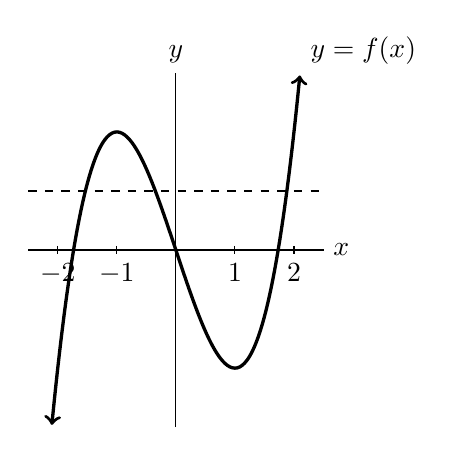
\begin{tikzpicture}[scale = .75]
\draw[very thick,<->] plot[smooth,samples=100,domain=-2.1:2.1](\x,{(\x)^3-3*(\x)}) node[above right]{$y=f(x)$};
\draw (-2.5,0)--(2.5,0) node[right]{$x$};
\draw (0,-3)--(0,3) node[above]{$y$};
\draw[dashed] (-2.5,1)--(2.5,1);
\foreach \x in{-2,-1,1,2}
	\draw (\x,2pt)--(\x,-2pt) node[below]{$\x$};
\end{tikzpicture}
\end{center}
\item Find the extrema on the graph provided.
\begin{center}
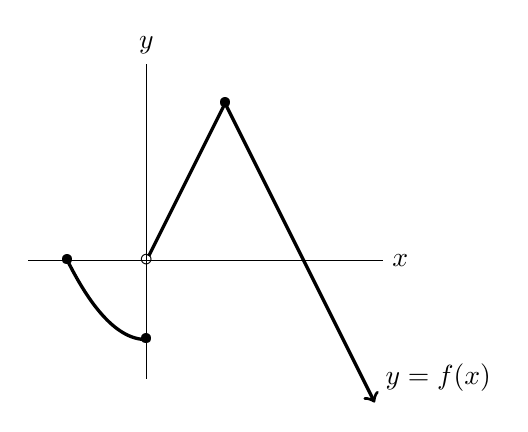
\begin{tikzpicture}
\draw[very thick] plot[smooth,samples=100,domain=-1:-0.05](\x,{(\x)^2-1});
\draw[very thick] plot[smooth,samples=100,domain=0.03:0.99](\x,{2*(\x)});
\draw[very thick,->] plot[smooth,samples=100,domain=1.01:2.9](\x,{-2*(\x)+4}) node[above right]{$y=f(x)$};
\node at (0,0) {$\circ$};
\node at (0,-1) {\textbullet};
\node at (1,2) {\textbullet};
\node at (-1,0) {\textbullet};
\draw (-1.5,0)--(3,0) node[right]{$x$};
\draw (0,-1.5)--(0,2.5) node[above]{$y$};
\end{tikzpicture}
\end{center}
\item A wave: \begin{tikzpicture}\draw plot[domain=0:6.28](\x,{sin(\x r)});\draw (0,0)--(6.5,0);\draw (0,-1.2)--(0,1.2);\end{tikzpicture}
\end{enumerate}
\noindent
\horrule{2pt} \\[0.1cm]
\noindent \textbf{STOP HERE!} Then $r(\theta)=\sin{\theta}+\cos{\theta}$ and $y=x\sqrt{2+x}$.
\end{document}
